\documentclass{article}
\usepackage[pdftex]{graphicx,color}
\usepackage[T1]{fontenc}
\usepackage{lmodern}
\usepackage{amsmath}
\usepackage{amsfonts}
\usepackage{subfigure}
\usepackage{textpos}

% use a larger page size; otherwise, it is difficult to have complete
% code listings and output on a single page
\usepackage{fullpage}

% have an index. we use the imakeidx' replacement of the 'multind' package so
% that we can have an index of all run-time parameters separate from other
% items (if we ever wanted one)
\usepackage{imakeidx}
\makeindex[name=prmindex, title=Index of run-time parameter entries]
\makeindex[name=prmindexfull, title=Index of run-time parameters with section names]
% be able to use \note environments with a box around the text
\usepackage{fancybox}
\newcommand{\note}[1]{
{\parindent0pt
  \begin{center}
    \shadowbox{
      \begin{minipage}[c]{0.9\linewidth}
        \textbf{Note:} #1
      \end{minipage}
    }
  \end{center}
}}

% use the listings package for code snippets. define keywords for prm files
% and for gnuplot
\usepackage{listings}
\lstset{
  language=C++,
  showstringspaces=false,
  basicstyle=\small\ttfamily,
  columns=fullflexible,
  keepspaces=true,
  frame=single,
  breaklines=true,
  postbreak=\raisebox{0ex}[0ex][0ex]{\hspace{5em}\ensuremath{\color{red}\hookrightarrow\space}}
}
\lstdefinelanguage{prmfile}{morekeywords={set,subsection,end},
                            morecomment=[l]{\#},escapeinside={\%\%}{\%},}
\lstdefinelanguage{gnuplot}{morekeywords={plot,using,title,with,set,replot},
                            morecomment=[l]{\#},}


% use the hyperref package; set the base for relative links to
% the top-level aspect directory so that we can link to
% files in the aspect tree without having to specify the
% location relative to the directory where the pdf actually
% resides
\usepackage[colorlinks,linkcolor=blue,urlcolor=blue,citecolor=blue,baseurl=../]{hyperref}

\newcommand{\dealii}{{\textsc{deal.II}}}
\newcommand{\pfrst}{{\normalfont\textsc{p4est}}}
\newcommand{\trilinos}{{\textsc{Trilinos}}}
\newcommand{\petsc}{{\textsc{PETSc}}}
\newcommand{\aspect}{\textsc{ASPECT}}

\begin{document}

\subsubsection{Inner core convection}
\label{sec:cookbooks-inner-core-convection}

\textit{This section was contributed by Juliane Dannberg, and the model setup was inspired 
by discussions with John Rudge.}

This is an example of convection in the Earth's inner core. The model is based on a spherical geometry. Three main particularities are constitutive of this inner core dynamics modelling: it consists of a self-gravitating sphere where the gravity increases linearly from zero at the center; the boundary conditions are permeable (material can cross the inner core boundary. See \cite{Deguen2013}); it's characterized by a single material with temperature dependent density that makes it unstably stratified as temperature increases towards the center of the core.

The setup is analogous to the models described in \cite{Deguen2013}, and all material properties 
are chosen in a way so that the equations are non-dimensional.

The required heating model and changes to the material model are implemented in a shared library
(\url{cookbooks/inner_core_convection/inner_core_convection.cc}). 

In their non-dimensional form, the equations are

\begin{align}
  \label{eq:inner-core-1}
  \nabla \cdot \sigma &=
  -Ra T \mathbf g,
  \\
  \label{eq:inner-core-2}
  \nabla \cdot \mathbf u &= 0,
  \\
  \label{eq:inner-core-3}
  \left(\frac{\partial T}{\partial t} + \mathbf u\cdot\nabla T\right)
  - \nabla^2 T
  &=
  H,
\end{align}

where $Ra$ is the Rayleigh number and $H$ is the 'source term'. The term $H$ is an artificial one, that arises from the time-variation of the adiabatic temperature in the outer core. Following \citet{Deguen2013}, with the proposed adimensionalization, $H=6$. 

\vspace{0.3cm}
\textbf{Thermal evolution of the inner core.}
During the Earth evolution, the temperature in the core decreases due to secular cooling. The isentropic temperature profile is used as a reference temperature, and when making the equations non-dimensional, a term emerges in the energy conservation equation, mathematically similar to a source term. The dimensional value of this source term is used in the Rayleigh number, as it is in the temperature scale. A slow time-variation of the adiabatic temperature will be associated to a negative source term, and a strongly stratified inner core ($Ra<0$). A positive value will be associated to a positive $Ra$ number, which indicates a convectively unstable inner core if the Rayleigh number is large enough. 


\vspace{0.3cm}
\textbf{Mechanical boundary.}
The mechanical boundary conditions for the inner core are
tangential stress-free and continuity of the normal stress at the
inner-outer core boundary. The inner core boundary is a freezing/melting boundary, and thus can't be considered completely impermeable. For the non-dimensional equations, that
means that we can define a ``phase change number'' $\mathcal{P}$ so that the
normal stress at the boundary is $-\mathcal{P} u_r$ with the radial velocity
$u_r$. This number characterizes the resistance to phase change at
the boundary, with $\mathcal{P}\rightarrow\infty$ corresponding to infinitely slow
melting/freezing (or a free slip boundary), and $\mathcal{P}\rightarrow0$ corresponding to
instantaneous melting/freezing (or a zero normal stress, corresponding to an open boundary).

In the weak form, this results in boundary conditions of the form
of a surface integral:
\begin{equation*}
\int_S \mathcal{P} (\mathbf u \cdot \mathbf n) (\mathbf v \cdot \mathbf n) dS,
\end{equation*}
with the normal vector $\mathbf n$.

This phase change term is added to the matrix in the 
\url{cookbooks/inner_core_convection/inner_core_assembly.cc} plugin by using a signal 
(as described in Section~\ref{sec:extending-signals}). The signal 
connects the function \verb!set_assemblers_phase_boundary!, which is only called once at the beginning of 
the model run. It creates the new assembler \texttt{PhaseBoundaryAssembler} for the boundary faces of the Stokes 
system and adds it to the list of assemblers executed in every time step. 
The assembler contains the function \verb!phase_change_boundary_conditions! that loops over all faces at the model 
boundary, queries the value of $\mathcal{P}$ from the material model, and adds the surface integral given above
to the matrix:
\lstinputlisting[language=C++,,basicstyle=\footnotesize\ttfamily,]{../../cookbooks/inner_core_convection/inner_core_assembly.cc}
Instructions for how to compile and run models with a shared library are given in Section~\ref{sec:benchmark-run}.

\vspace{0.3cm}
\textbf{Governing parameters.} Analyzing Equations~\eqref{eq:inner-core-1}--\eqref{eq:inner-core-3} reveals that two parameters determine the dynamics of convection in the inner core: the Rayleigh number $Ra$ and the phase change number $\mathcal{P}$. Three main areas can be distinguished: the stable area, the plume convection area and the translation mode of convection area (Figure~\ref{fig:diagramme-regime}). For low Rayleigh numbers (below the critical value $Ra_c$), there is no convection and thermal diffusion dominates the heat transport. However, if the inner core is convectively unstable ($Ra$>$Ra_c$), the convection regime depends mostly on $\mathcal{P}$. For low $\mathcal{P}$ (<29), the convective translation mode dominates, where material freezes at one side and melts at the other side, so that the velocity field is uniform, pointing from the freezing to the melting side. Otherwise, at high $\mathcal{P}$ (>29), convection takes the usual form of plume convection. In this case, there is almost no melting or solidification associated with this mode. At intermediate values of P, the first unstable mode is a linear combinaison of the high-$\mathcal{P}$ convection mode and of the small-$\mathcal{P}$ translation mode.

\begin{figure}[h]
\begin{center}
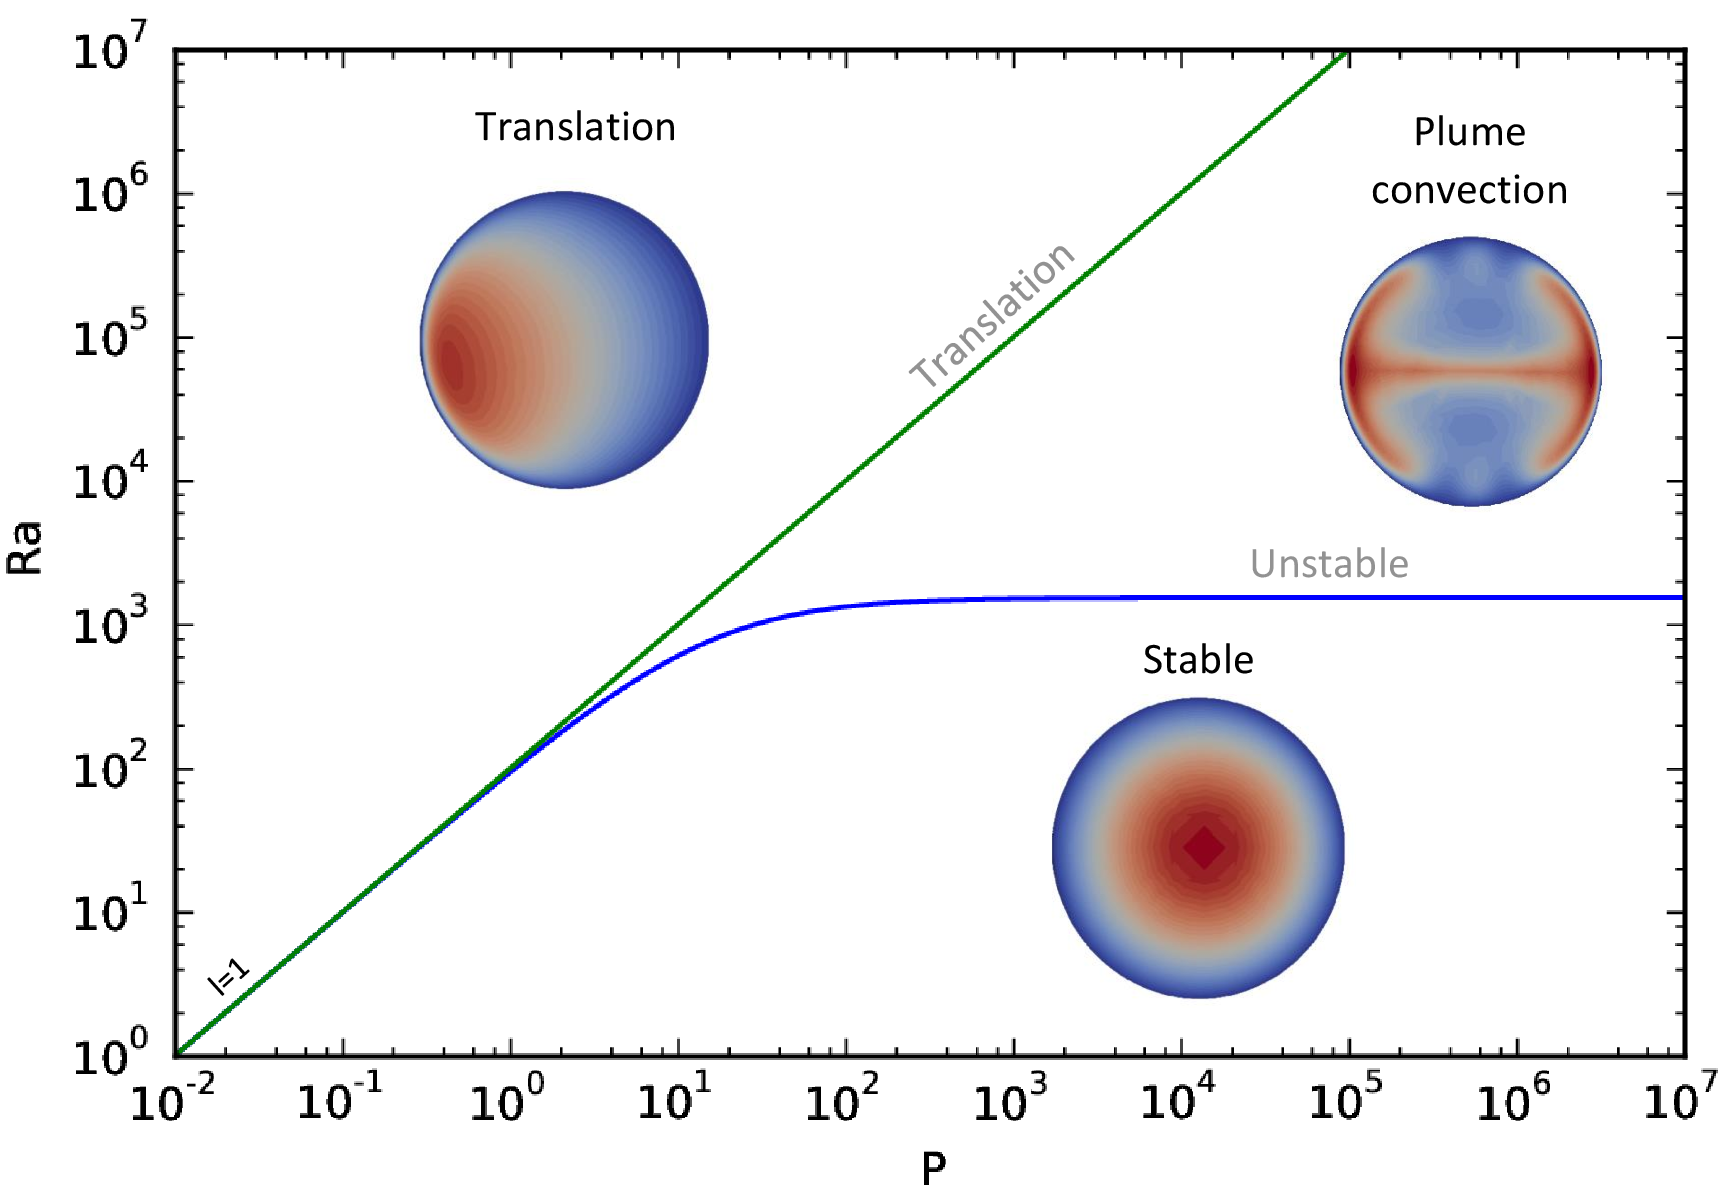
\includegraphics[height=0.57\textwidth]{cookbooks/inner_core_convection/Diagstab.png}
\caption{Stability diagram for convection in a sphere with phase change at its outer boundary. The stability curves for the first unstable mode (l=1) and the translation are obtained from \cite{Deguen2013}.}
    \label{fig:diagramme-regime}
\end{center}
\end{figure}

Changing the values of $Ra$ and $\mathcal{P}$ in the input file allows switching between the different regimes.
The Rayleigh number can be changed by adjusting the magnitude of the gravity:
\lstinputlisting[language=prmfile]{cookbooks/inner_core_convection/inner_core_traction.part.2.prm}
The phase change number is implemented as part of the material model, and as a function that can depend on the 
spatial coordinates and/or on time: 
\lstinputlisting[language=prmfile]{cookbooks/inner_core_convection/inner_core_traction.part.1.prm}

Figure~\ref{fig:inner-core-regimes} shows examples of the three regimes with $Ra=10^5, \mathcal{P}=10^4$ (plume convection), 
$Ra=10^2, \mathcal{P}=10^-1$ (translation), $Ra=1, \mathcal{P}=1$ (no convection).

\begin{figure}[h]
    \begin{center}
    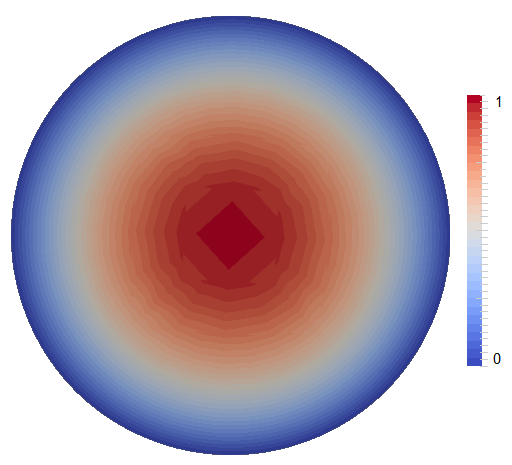
\includegraphics[width=0.25\linewidth]{cookbooks/inner_core_convection/Ra1e0P0modif.png}
    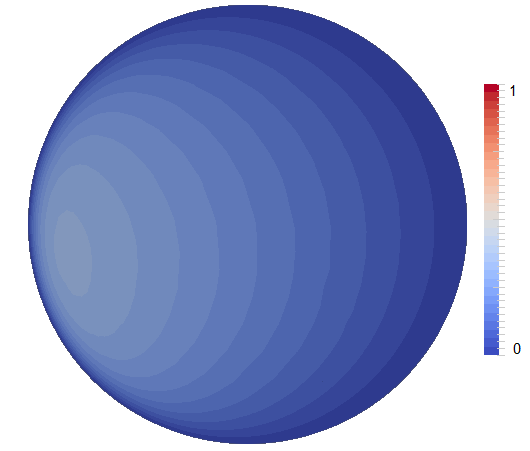
\includegraphics[width=0.25\linewidth]{cookbooks/inner_core_convection/Ra1e2P-1modif.png}
    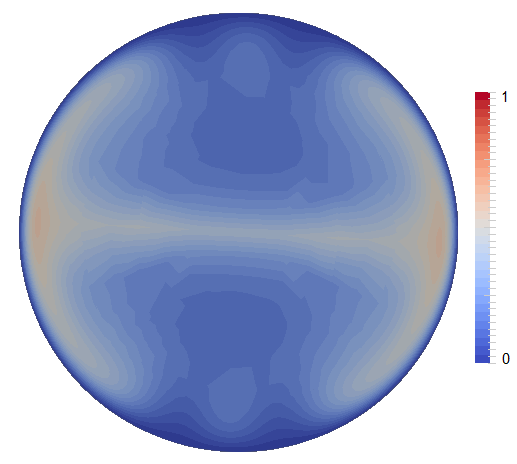
\includegraphics[width=0.25\linewidth]{cookbooks/inner_core_convection/Ra1e5P4modif.png}
   \vspace{1cm}
    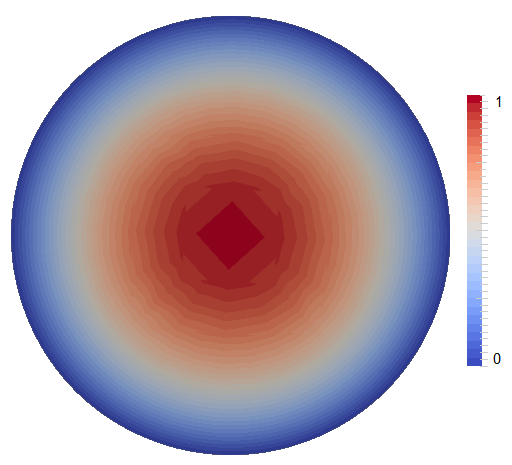
\includegraphics[width=0.25\linewidth]{cookbooks/inner_core_convection/Ra1e0P0modif.png}
    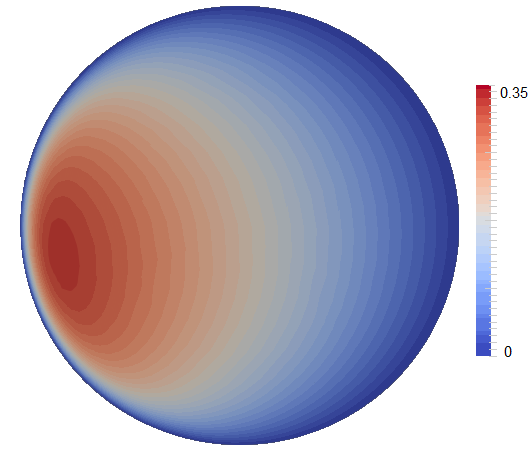
\includegraphics[width=0.25\linewidth]{cookbooks/inner_core_convection/Ra1e2P-1rescalemodif.png}
    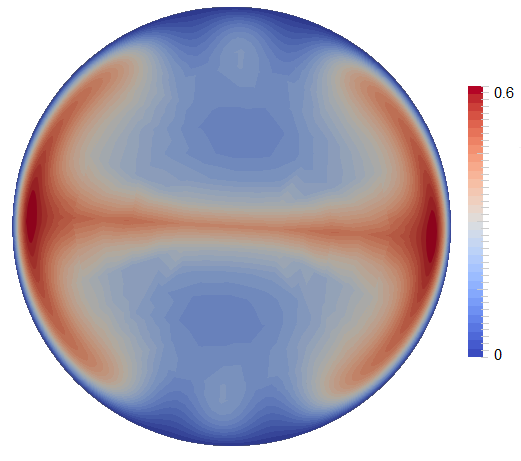
\includegraphics[width=0.25\linewidth]{cookbooks/inner_core_convection/Ra1e5P4rescalemodif.png}
    \caption{Convection regimes in the inner core for different values of $Ra$ and $\mathcal{P}$. From left to right: no convection, translation, plume convection; the 2D slices of the top are with the default temperature scale while at the bottom an adaptative scale is used.}
    \label{fig:inner-core-regimes}
       \end{center}
\end{figure}

\vspace{0.3cm}
\textbf{Mesh refinement.}
In the particular case of the inner core dynamics, two main type of mesh refinement could be used. For simulations in the translative mode (Figure 1 ), the particular boundary implies that a finest refinement at the outer boundary is more appropriate. The boundary is permeable, allowing melting or freezing and transfer of material through the boundary. The temperature is set at 1 et the boundary, and for the translation case, a large temperature gradient is imposed at the boundary layer. For this, a specific refinement has to be set for defining correctly the boundary layer at the inner core boundary. For simulations in plume convection, an adaptative mesh-refinement (with the temperature field for exemple) is more adapted, otherwise, the plumes are not enough defined.

In order to have a mesh that is much finer at the outer boundary than in the center of the domain, this expression for the mesh refinement subsection can be used in the input file :
\lstinputlisting[language=prmfile]{cookbooks/inner_core_convection/inner_core_traction.part.3.prm}

The sum of the "Initial global refinement" and the "Initial adaptative refinement" is always the maximum refinement of the model. In order to have a finest mesh with a refinement of 6 (like for the exemple above), the sum of those two parameters should be 6. The "Initial global refinement" is used to start with an uniform mesh, and then it does a number of mesh refinement step equal to the "Initial adaptive refinement". For higher Rayleigh numbers, the mesh has to be better refine, especially in the thermal boundary layers. This can be achieve by   changing the first term in the parenthesis, which corresponds to the pourcentage of the sphere you want to have a better refinment. 

\vspace{0.3cm}
\textbf{Scaling laws.} In addition, \cite{Deguen2013} give scaling laws for the velocities in each regime derived from linear stability analysis, and show how numerical results compare to them. In the regimes of low $\mathcal{P}$, translation will start 
at a critical ratio of Rayleigh number and phase change number $\frac{Ra}{\mathcal{P}}=\frac{175}{2}$ with steady-state 
translation velocities being zero below this threshold and tending to $v_0=\frac{175}{2}\sqrt{\frac{6}{5}\frac{Ra}{\mathcal{P}}}$ 
going towards higher values of $\frac{Ra}{\mathcal{P}}$.
In the same way, translation velocities will decrease from $v_0$ with increasing $\mathcal{P}$, with translation transitioning
to plume convection at $\mathcal{P}\sim29$. 
Both trends are shown in Figure~\ref{fig:inner-core-trends} and can be compared to Figure~8 and 9 in \cite{Deguen2013}.
 
\begin{figure}
    \centering
    \includegraphics[width=0.49\textwidth]{cookbooks/inner_core_convection/translation_over_Ra_P.pdf}
    \hfill
    \includegraphics[width=0.49\textwidth]{cookbooks/inner_core_convection/translation_over_P.pdf}
    \caption{Translation rate (approximated by the average of the velocity component in the direction of translation), 
    normalized to the low $\mathcal{P}$ 
    limit estimate given in \cite{Deguen2013}, as a function of $\frac{Ra}{\mathcal{P}}$ for $\mathcal{P}=10^{-2}$ 
    (left) and as a function of $\mathcal{P}$ for $Ra=10^5$ (right).
    The dashed gray line gives the translation velocity predicted in the limit of low $\mathcal{P}$. Disagreement 
    for larger values of $\mathcal{P}$ indicates that higher order terms (not included in the low $\mathcal{P}$
    approximation) become important. Additionally, differences between the analytical and numerical model might 
    be the result of limited resolution (only 12 elements in radial direction).}
    \label{fig:inner-core-trends}
\end{figure}

\end{document}